\documentclass[12pt,a4paper]{article}
\usepackage[utf8]{inputenc}
\usepackage[russian]{babel}
\usepackage[OT1]{fontenc}
\usepackage{amsmath}
\usepackage{amsfonts}
\usepackage{amssymb}
\usepackage{graphicx}
\usepackage{array}
\usepackage{cancel}
\usepackage{caption}
\usepackage{wrapfig}
\usepackage[left=1.5cm,right=1.5cm,top=0.3cm,bottom=1.5cm,includefoot,footskip=1.5cm]{geometry}
\begin{document}
\textbf{
\begin{flushright}
Илья Кочергин, 626 группа
\end{flushright}}
\begin{flushleft}
\large\textbf{Работа 3.2.6}
\medskip

\Large\textbf{Исследование гальванометра}
\end{flushleft}

\noindent\textbf{Цель работы:} изучение работы высокочувствительного магнитозеркального гальванометра магнитоэлектрической системы в режимах измерения постоянного тока и электрического заряда.
\medskip

\noindent\textbf{Оборудование:} зеркальный гальванометр с осветителем и шкалой, источник постоянного напряжения, делитель напряжения, магазин сопротивлений, эталонный конденсатор, вольтметр, переключатель, ключ, линейка.

\paragraph{\large 1.}\large\textbf{Теоретическая справка}\normalsize
\medskip

\begin{wrapfigure}{r}{0.23\textwidth}
\centering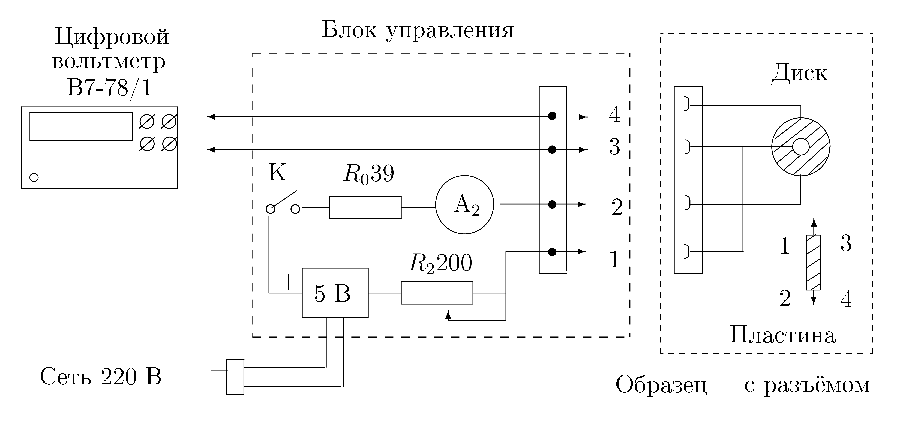
\includegraphics[width = 0.17\textwidth]{Pct1}
\captionsetup{justification = centering}
\caption{Рамка с током в магнитном поле \label{Fig1}}
\end{wrapfigure}
\textbf{Устройство.} Баллистический гальванометр - электроизмериткльный прибор магнитоэлектроической системы, отличающийся высокой чувствительностью и сравнительно большим периодом колебвний подвижной части. Он представляет собой скрепленную с полым цилиндром проводящую рамку, подвешенную на нити в радиально направленном постоянном магнитном поле (см. рис. \ref{Fig1}). На рамке закреплено зеркало, служащее для измерения угла поворота.
\medskip

\textbf{Уравнение движения.} Введем следующие обозначения: $\varphi$ - угол поворота рамки, $D$ - модуль кручения, $S$ - площадь рамки, $N$ - число витков, $I$ - сила тока в рамке при отсутствии ЭДС индукции, $B$ - индукция магниного поля, $R_{\Sigma}$ - общее сопротивление цепи, $J$ - момент инерции подвижной системы. Если пренебречь сопротивлением воздуха, то уравнение движения записывается в виде
\begin{equation}
J\ddot\varphi + \frac{(BSN)^2}{R_{\Sigma}}\dot\varphi + D\varphi = BSNI\label{em}.
\end{equation}
Введем обозначения
\begin{equation}
\begin{cases}
2\gamma = \frac{(BSN)^2}{JR_{\Sigma}},\\
\omega_0^2 = \frac{D}{J},\\
K = \frac{BSN}{J}.\\
\end{cases}
\end{equation}
Таким образом, уравнение (\ref{em}) примет вид
\begin{equation}
\ddot\varphi + 2\gamma\dot\varphi + \omega_0^2\varphi = KI\label{emm}.
\end{equation}
Заметим, что данное уравнения является уравнением затухающих колебаний с коэффициентом затухания $\gamma$ и собственной частотой $\omega_0$.
\medskip

\textbf{Режим измерения постоянного тока.} Если $I = const$, то по прошествии некоторого времени колебания затухнут, и можно принять $\varphi = const$. Тогда из уравнения (\ref{emm}) легко получить
\begin{equation}
\varphi = \frac{K}{\omega_0^2}I = \frac{BSN}{D}I = \frac{I}{C_I}.
\end{equation}
$C_I$ называется \textit{динамической постоянной} гальванометра и определяется выражением
\begin{equation}
C_I = \frac{I}{\varphi} = \frac{D}{BSN}.\label{dyn}
\end{equation}
\medskip

\textbf{Свободные колебания рамки.} Пусть $I = 0$ и выполнены следующие начальные условия:
\begin{equation}
\begin{cases}
\varphi(t = 0) = 0,\\
\dot\varphi(t = 0) = \dot\varphi_0.\\
\end{cases}
\end{equation}
Тогда в зависимости от $\gamma$ и $\omega_0$ решение уравнения (\ref{emm}) имеет вид
\begin{equation}
\begin{cases}
\varphi = \frac{\dot\varphi_0}{\omega}e^{-\gamma t}\sin\omega t,&\gamma < \omega_0~\text{(колебательный режим)};\\
\varphi = \frac{\dot\varphi_0}{\omega_0}\sin\omega_0 t,&\gamma = \omega_0~\text{(критический режим)};\\
\varphi = \frac{\dot\varphi_0}{\varkappa}e^{-\gamma t}\sh\varkappa t,&\gamma > \omega_0~\text{(апериодический режим)}.\\
\end{cases}\label{sol}
\end{equation}
Здесь $\varkappa$ и $\omega$ определяются соотношениями
\begin{equation}
\begin{cases}
\omega^2 = \omega_0^2 - \gamma^2,\\
\varkappa^2 = \gamma^2 - \omega_0^2.\\
\end{cases}
\end{equation}

В случае колебательного режима можно ввести логарифмический декремент затухания $\Theta$:
\begin{equation}
\Theta = \ln\frac{\varphi_n}{\varphi_{n+1}},
\end{equation}
где $\varphi_n$ и $\varphi_{n+1}$ - углы последовательных отклонений в одну сторону с номерами $n$ и $n+1$. Из (\ref{sol}) в случае малого затухания ($\gamma \ll \omega$) легко получить выражение для $\Theta$:
\begin{equation}
\Theta = \gamma T\label{decr},
\end{equation}
где $T$ - период колебаний:
\begin{equation}
T = \frac{2\pi}{\omega}\label{per}.
\end{equation}
Заметим, что при приближении к критическому режиму $\Theta \to \infty$.
\medskip

\textbf{Режим измерения заряда.} Теперь рассмотрим ситуацию, когда через гальванометр проходит короткий импульс тока. Будем считать, что продолжительность импульса $\tau$ достаточно мала ($\tau \ll T$), и отклонением рамки можно пренебречь. Пусть через рамку протекал ток с момента времени $t = 0$ до момента времени $t = \tau$. Проинтегрировав уравнение (\ref{emm}) с учетом приближения $\varphi \approx 0$, получим
\begin{equation}
\dot\varphi(\tau) = K\int\limits_0^\tau Idt\label{dotphi1}.
\end{equation}
Заряд, прошедший через гальванометр выражается формулой
\begin{equation}
q = \int\limits_0^\tau Idt + \int\limits_0^\tau I_{\text{инд}}dt\label{ch},
\end{equation}
где $I_{\text{инд}}$ - индукционный ток. Заметим, что $I_{\text{инд}} \sim \dot\varphi$, а значит
\begin{equation}
\int\limits_0^\tau I_{\text{инд}}dt \sim \int\limits_0^\tau \dot\varphi dt = \varphi(\tau) \approx 0.
\end{equation}
Поэтому зарядом, протекшим в результате индукционного тока, можно пренебречь, и выражение (\ref{ch}) примет вид
\begin{equation}
q = \int\limits_0^\tau Idt.
\end{equation}
Отсюда и из выражения (\ref{dotphi1}) получим
\begin{equation}
\dot\varphi(\tau) = Kq\label{dotphi2}.
\end{equation}
Из выражения (\ref{sol}) легко видеть, что при любом режиме максимальное отклонение от положения равновесия $\varphi_\text{max} \sim \dot\varphi_0 \stackrel{(\ref{dotphi2})}{\sim} q$. Таким образом, величина
\begin{equation}
C_q = \frac{q}{\varphi_\text{max}}\label{bal},
\end{equation}
называемая \textit{баллистической постоянной}, зависит только от параметров цепи.

Можно показать, что при неизменном $q$ максимальное отклонение достигается при отсутствии затухания и определяется выражением
\begin{equation}
\varphi_{\text{max св}} = \frac{\dot\varphi(\tau)}{\omega_0} = \frac{Kq}{\omega_0}\label{fr}.
\end{equation}
В критическом режиме, когда система быстрее всего приходит в равновесие, максимальное отклонение в $e$ раз меньше:
\begin{equation}
\varphi_{\text{max кр}} = \frac{Kq}{\omega_0e}\label{cr}.
\end{equation}
Отсюда следует выражение для баллистических констант:
\begin{equation}
\frac{C_{Q\text{ кр}}}{C_{Q\text{ св}}} = e\label{rat}.
\end{equation}

\paragraph{\large 2.}\large\textbf{Определение динамической постоянной}\normalsize
\medskip

\begin{wrapfigure}{r}{0.5\textwidth}
\centering\includegraphics[width = 0.47\textwidth]{Sch1}
\captionsetup{justification = centering}
\caption{Схема установки для работы в стационарном режиме \label{Fig2}}
\end{wrapfigure}
\textbf{Экспериментальная установка.} Схема для измерений в стационарном режиме приведена на рис. \ref{Fig2}. Значение входного напряжения $U = 1,32 \pm 0,02~\text{В}$, сопротивления гальванометра $R_0 = 475 \pm 1~\text{Ом}$. Сопротивление $R$ можно изменять.

Угол отклонения рамки от пложения равновесия измеряется с помощью осветителя, зеркала, закрепленного на рамке, и шкалы, на которую отражается свет. Если обозначить координату светового пятна за $x$ и считать $x \ll a$, то выражение для угла отклонения примет вид
\begin{equation}
\varphi = \frac{x}{2a},
\end{equation}
где $a = 128 \pm 1~\text{см}$ - расстояние от шкалы до зеркала. Таким образом, из выражения (\ref{dyn}) легко получить формулу для динамической постоянной:
\begin{equation}
C_I = \frac{2aI}{x} 
\end{equation}
Отсюда следует выражение для зависимости $I(x)$:
\begin{equation}
I = x\frac{C_I}{2a}\label{dyn_rel}.
\end{equation}

При $R_1 \ll R + R_0$ сила тока, протекающего через гальванометр, выражается формулой
\begin{equation}
I = U\frac{R_1}{R_2}\frac{1}{R + R_0}.
\end{equation}
По этой формуле мы можем рассчитать токи по значениям сопротивления $R$, и, таким образом, получить экспериментальную зависимость $I(x)$. Согласно (\ref{dyn_rel}), она должна быть линейной, и по ее коэффициенту наклона $k$ мы сможем вычислить $C_I$:
\begin{equation}
C_I = 2ka.
\end{equation}


\end{document}